\section{\ac{lorawan}}\label{sec:lorawanADR}
\ac{lorawan} is a MAC layer protocol designed to be the de facto choice for point-to-multipoint \ac{lora} applications. It is largely certified worldwide, open-source, and is both managed and promoted by the LoRa Alliance\footnote{Lora Alliance,  https://lora-alliance.org/}. The expectation of a star topology means the full protocol is not suited to the sparse swarm scenario, however, individual features are of interest. In principle it is implemented as Pure ALOHA (P-ALOHA) - a simple unchecked protocol where transmission occurs whenever a transmitter has data available to send. Figure \ref{fig:lorawan_duty_cycles} explains how duty cycle limits are enforced. The unchecked approach reduces theoretical channel usage to just 18\% \cite{3YP:LORAWAN_SLOTTED}. \ac{lorawan} abstracts \ac{sf}s and \ac{bw}s into a set of orthogonal data-rates where lower data-rates have higher range \cite{3YP:LORAWAN_REGIONAL_PARAMS}.

\begin{figure}[H]
    \centering
   	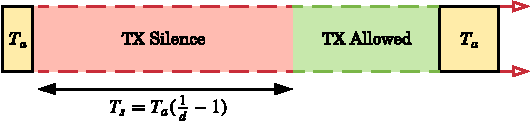
\includegraphics{Figures/duty_cycle_lorawan.pdf}
    \caption[\ac{lorawan} duty cycle enforcement]{
    Demonstration of how \ac{lorawan} enforces duty cycle limits; that is after a transmission of airtime $T_a$, the transmitter must be silent for a minimum period of $T_s=T_a(\frac{1}{d_c}-1)$ \cite{3YP:LIMITS_OF_LORAWAN}. The figure is to scale for $d_c=10\%$.
    
    }
    \label{fig:lorawan_duty_cycles}
\end{figure}


Optionally, \ac{tp}, \ac{sf} and \ac{bw} can be managed dynamically using \ac{lorawan}'s adaptive data-rate (ADR) functionality. Full technical detail is available in \cite{3YP:LORAWAN}, a brief overview follows. Operation is scheduled by a node setting the reserved \ac{adr} bit in uplink messages. The gateway responds with initial transmission parameters to attempt. The node sets its transmission parameters to these values and proceeds with the expectation that the gateway is reachable. However, if the gateway does not acknowledge any packets within a set period, the \ac{adr} bit is set again to force an acknowledgement. Failure to receive any acknowledgement implies that the gateway is not within range. Data-rate is reduced or \ac{tp} is increased until an acknowledgement is made, these are the parameters used unless a further \ac{adr} request is made. It has been suggested that the system has low-scalability due to packet count requirements \cite{3YP:LORAWAN_ADR} and is slow to converge \cite{3YP:LORAWAN_ADR_AGILITY}. Like \cite{3YP:CHOOSING_LORA_PARAMETERS}, this makes it only suitable for static nodes in a gateway controlled network.